\section{Metodología}
\label{sec:metodologia}

El trabajo se enmarca en una investigación de tipo aplicada, orientada al diseño y construcción de una arquitectura de sistema de Reconocimiento Automático de Matrículas (ANPR) para la gestión de parqueaderos. El énfasis no está únicamente en la evaluación de un algoritmo de visión por computador, sino en la definición y validación de un conjunto de componentes que, integrados, permiten automatizar el registro de vehículos y servir como plataforma de experimentación en contextos académicos.

La investigación se desarrolló en el marco de un trabajo de grado del Servicio Nacional de Aprendizaje (SENA), dentro de un programa de formación en análisis y desarrollo de software. Por tanto, la metodología combina elementos de ingeniería de software (levantamiento de requisitos, diseño arquitectónico, implementación y pruebas) con una intención formativa: consolidar y poner en práctica conceptos de visión por computador, microservicios, mensajería distribuida y desarrollo web y móvil.

La metodología se estructura en cuatro fases principales:

\begin{enumerate}
    \item Análisis del contexto y definición de requisitos.
    \item Diseño de la arquitectura propuesta.
    \item Implementación del caso de estudio ANPR-VISION.
    \item Evaluación inicial y reflexión sobre resultados y extensiones posibles.
\end{enumerate}

A continuación se describen en detalle cada una de estas fases, así como las tecnologías y conceptos investigados y aplicados en el proceso.

\subsection{Fase 1: Análisis del contexto y definición de requisitos}

En la primera fase se realizó un análisis del contexto de uso al que se orienta el sistema: parqueaderos de pequeña y mediana escala, típicos de instituciones educativas, conjuntos residenciales y organizaciones que gestionan el acceso de vehículos de manera manual o con sistemas parcialmente automatizados. Este análisis se apoyó tanto en la observación de prácticas reales como en la revisión de trabajos relacionados en ANPR, aparcamiento inteligente y ciudades inteligentes (Sección~\ref{sec:relacionados}).

A partir de esta revisión se definió un conjunto de requisitos funcionales y no funcionales:

\begin{itemize}
    \item \textbf{Registro automático de entradas y salidas}: el sistema debe ser capaz de detectar la entrada y salida de vehículos en puntos de acceso determinados, asociando a cada evento la matrícula reconocida, la hora y la cámara de origen.
    \item \textbf{Uso de tecnologías abiertas}: todos los componentes (modelos de visión, microservicios, bases de datos, frontends) deben construirse con herramientas de código abierto, de modo que el sistema pueda ser estudiado, modificado y desplegado sin licencias propietarias.
    \item \textbf{Arquitectura modular}: la solución debe organizarse en componentes claramente diferenciados (visión, mensajería, gestión de parqueaderos, interfaces de usuario), para facilitar su comprensión y su posible sustitución o ampliación.
    \item \textbf{Procesamiento en tiempo casi real}: aunque el sistema se desarrolla con fines educativos, la latencia entre la detección de un vehículo y la notificación al usuario debe ser compatible con la operación normal de un parqueadero.
    \item \textbf{Persistencia y consulta de información}: el sistema debe permitir almacenar los registros de visitas y ponerlos a disposición de las interfaces web y móviles para consulta posterior por parte de administradores y usuarios.
    \item \textbf{Escenario de validación controlado}: el prototipo debe poder desplegarse en un entorno de prueba que replique, a pequeña escala, el comportamiento de un parqueadero real, con cámaras reales o flujos de video de prueba.
\end{itemize}

Estos requisitos orientan las decisiones de diseño y acotan el alcance del proyecto: no se busca reemplazar soluciones comerciales completas, sino construir una arquitectura clara, replicable y adecuada para experimentación y formación.

\subsection{Fase 2: Diseño de la arquitectura propuesta}

La segunda fase se centró en el diseño de la arquitectura de sistema. A partir de los requisitos anteriores y de la literatura consultada, se optó por una organización basada en microservicios y en mensajería distribuida, separando explícitamente la capa de visión de la lógica de gestión de parqueaderos.

En términos generales, se definieron los siguientes componentes:

\begin{enumerate}
    \item \textbf{Microservicio de visión (Python)}: responsable de recibir flujos de video desde cámaras IP o archivos de prueba, aplicar los modelos de detección y reconocimiento de matrículas y generar eventos estructurados.
    \item \textbf{Bus de mensajería (Apache Kafka)}: encargado de recibir los eventos generados por el microservicio de visión y distribuirlos a los servicios consumidores; actúa como capa de desacoplamiento entre la visión y el backend de gestión.
    \item \textbf{Sistema de gestión de parqueaderos (backend .NET)}: API que mantiene la información de vehículos, usuarios, tarifas, plazas y registros de visitas; consume los eventos de detección para actualizar el estado del parqueadero.
    \item \textbf{Interfaces de usuario (Angular y aplicación móvil)}: frontends que permiten al personal operativo visualizar en tiempo cercano al real las detecciones y gestionar el parqueadero, y que ofrecen al usuario final acceso a su historial de visitas y saldos.
    \item \textbf{Canal de notificación en tiempo cercano al real (SignalR)}: mecanismo para enviar mensajes desde el backend hacia los clientes web y móviles cuando se produce un nuevo evento relevante (por ejemplo, detección de una matrícula o cierre de una visita).
\end{enumerate}

Durante esta fase se elaboraron diagramas de componentes, de despliegue y de secuencia para representar la interacción entre los módulos. El microservicio de visión se concibió como un módulo autónomo capaz de procesar uno o varios flujos de video, mientras que el backend .NET se diseñó como la “fuente de verdad” en cuanto a la información de parqueaderos, vehículos y transacciones. Apache Kafka se ubicó en el centro de la arquitectura como canal principal de comunicación asíncrona, permitiendo que otros componentes futuros (por ejemplo, módulos de analítica avanzada) puedan suscribirse a los eventos sin modificar el microservicio de visión ni el backend existente.

En paralelo, se definieron las estructuras de datos que circulan entre los componentes, en particular el formato de los eventos de detección (matrícula, cámara, marca de tiempo, confianza, tipo de evento, etc.) y los modelos manejados en el backend (vehículos, visitas, usuarios, tarifas).

\subsection{Fase 3: Implementación del microservicio de visión}

La tercera fase se centró en la construcción del microservicio de visión, implementado en Python. Esta fase incluyó el estudio y selección de los modelos y bibliotecas a utilizar, así como la integración de estos dentro de una canalización de procesamiento coherente.

Los principales elementos tecnológicos y conceptuales considerados fueron:

\begin{itemize}
    \item \textbf{Detección de vehículos y matrículas con YOLOv5}: se adoptó un modelo de la familia \textit{YOLOv5} entrenado para detectar vehículos y, en algunos casos, regiones de matrícula. Este tipo de modelos ofrece un equilibrio adecuado entre precisión y velocidad para aplicaciones en tiempo casi real, y cuenta con implementaciones y ejemplos de código abierto ampliamente documentados.
    \item \textbf{Localización de la región de la placa}: en los casos en que el modelo de detección entrega solo la caja correspondiente al vehículo, se aplica un paso adicional para localizar la matrícula dentro de dicha región, utilizando heurísticas geométricas y, en ocasiones, modelos secundarios especializados en placas.
    \item \textbf{Reconocimiento óptico de caracteres (OCR) con EasyOCR}: para la lectura de los caracteres de la matrícula se emplea EasyOCR, una biblioteca de OCR de código abierto que soporta múltiples idiomas y ofrece un rendimiento suficiente para el prototipo. Se investigaron aspectos como la normalización de la imagen (escala de grises, contraste, filtrado) para mejorar la calidad del reconocimiento.
    \item \textbf{Seguimiento de objetos con ByteTrack}: con el fin de mantener la identidad del vehículo a lo largo del tiempo, se integró el algoritmo de seguimiento ByteTrack, que asocia detecciones consecutivas basándose en la posición y en la confianza de los cuadros delimitadores. Este seguimiento permite reducir lecturas duplicadas y estimar de manera más fiable el momento de entrada y de salida.
    \item \textbf{Gestión de flujos de video}: el microservicio se diseñó para recibir video a través de protocolos como RTSP o desde archivos de prueba, dividiendo el flujo en fotogramas (\textit{frames}) que se van procesando de manera secuencial. Se implementó una lógica para controlar la tasa de procesamiento (por ejemplo, procesar uno de cada varios fotogramas) y así equilibrar el consumo de recursos y la latencia.
\end{itemize}

Una vez procesados los fotogramas y reconocida la matrícula, el microservicio genera eventos estructurados que incluyen la información relevante para la capa de gestión. Estos eventos se envían a un tópico de Apache Kafka definido específicamente para detecciones de matrículas. La comunicación con Kafka se realiza mediante librerías de cliente de código abierto para Python, y se probaron diferentes configuraciones de producción (por ejemplo, tamaños de lote y políticas de reintento) en el entorno de pruebas.

Es importante señalar que, dado el carácter educativo del proyecto, la implementación se orientó a lograr un funcionamiento correcto y estable del microservicio en escenarios controlados, más que a exprimir al máximo el rendimiento del modelo o a realizar optimizaciones de bajo nivel. No obstante, la arquitectura permite sustituir el modelo de detección o la biblioteca de OCR por alternativas más avanzadas en trabajos futuros.

\subsection{Fase 4: Implementación del backend de gestión y de las interfaces de usuario}

En paralelo a la construcción del microservicio de visión, se desarrolló el sistema de gestión de parqueaderos y las interfaces de usuario.

\subsubsection{Backend de gestión (.NET)}

El backend se implementó utilizando .NET, siguiendo una organización por capas que separa la lógica de negocio, el acceso a datos y la exposición de la API. Entre los conceptos trabajados en esta fase se encuentran:

\begin{itemize}
    \item \textbf{Modelado de entidades}: diseño de modelos para representar vehículos, usuarios, parqueaderos, cámaras, visitas (entradas y salidas) y tarifas. Este modelado incluyó la definición de relaciones entre entidades (por ejemplo, un vehículo puede tener múltiples visitas, cada visita está asociada a un parqueadero y a una cámara de entrada).
    \item \textbf{API REST}: implementación de controladores para registrar y consultar las visitas, gestionar la configuración de parqueaderos y cámaras, y exponer los datos necesarios para las interfaces web y móviles.
    \item \textbf{Consumo de eventos desde Kafka}: desarrollo de un componente que se suscribe al tópico de detecciones del microservicio de visión, interpreta los eventos y actualiza la base de datos con nuevas entradas o salidas, según las reglas de negocio definidas.
    \item \textbf{Registro de eventos y auditoría}: incorporación de mecanismos de registro (\textit{logging}) para dejar trazas de las detecciones procesadas, las decisiones de apertura o cierre de visitas y los posibles errores, facilitando el análisis posterior.
\end{itemize}

El backend se planteó como la “fuente de verdad” respecto al estado del parqueadero, de modo que cualquier decisión de negocio (por ejemplo, calcular el tiempo de permanencia o el monto a pagar) se centraliza en este componente.

\subsubsection{Interfaces web y móviles}

Sobre el backend se construyeron dos tipos de interfaces:

\begin{itemize}
    \item \textbf{Portal web (Angular)}: orientado al personal operativo y a la administración del parqueadero. Permite visualizar en tiempo cercano al real las detecciones de matrículas, consultar el estado de ocupación de las plazas, revisar el historial de visitas y gestionar la configuración del sistema (cámaras, tarifas, usuarios, etc.).
    \item \textbf{Aplicación móvil}: dirigida al usuario final (propietario del vehículo), con el objetivo de que pueda consultar sus vehículos registrados, el historial de accesos al parqueadero y los saldos asociados. Esta aplicación actúa principalmente como cliente de consulta sobre la API del backend.
\end{itemize}

La comunicación en tiempo cercano al real entre el backend y las interfaces se implementó mediante SignalR, que permite establecer canales bidireccionales y enviar notificaciones a los clientes cuando se registra una nueva detección o se actualiza el estado de una visita. Se trabajó en la gestión de estos canales y en la actualización dinámica de las vistas del frontend.

\subsection{Fase 5: Integración y pruebas en entorno controlado}

Una vez implementados los componentes principales, se llevó a cabo una fase de integración en un entorno de pruebas. Para ello se utilizaron contenedores Docker y archivos \texttt{docker-compose} que facilitan el despliegue de los servicios (microservicio de visión, Kafka, backend y frontends) en una misma máquina o en una red local.

Las pruebas se realizaron inicialmente con flujos de video de prueba y, posteriormente, con cámaras IP en un entorno controlado que simula el acceso a un parqueadero. Los criterios observados incluyeron:

\begin{itemize}
    \item \textbf{Correctitud funcional}: verificación de que, al pasar un vehículo por el campo de visión de la cámara, el sistema detecta la matrícula, genera el evento correspondiente y registra la visita en la base de datos.
    \item \textbf{Consistencia de la información}: comprobación de que las matrículas reconocidas se mantienen coherentes a lo largo de la visita, evitando registros duplicados o inconsistentes.
    \item \textbf{Latencia observable}: estimación del tiempo transcurrido entre la captura del fotograma, el procesamiento en el microservicio de visión, la llegada del evento al backend y la actualización de las interfaces de usuario.
\end{itemize}

Dado que el proyecto tiene un alcance de trabajo de grado y se desarrolló con recursos limitados, no se realizó una evaluación estadística exhaustiva con grandes conjuntos de datos ni en condiciones ambientales extremas. Sin embargo, las pruebas en el entorno controlado permitieron comprobar la coherencia de la arquitectura y obtener información cualitativa sobre su comportamiento.

\subsection{Fase 6: Evaluación, limitaciones y oportunidades de ampliación}

La última fase de la metodología consiste en analizar críticamente los resultados obtenidos y en identificar las principales limitaciones y oportunidades de ampliación del sistema.

Entre las limitaciones observadas se encuentran:

\begin{itemize}
    \item La ausencia de una evaluación cuantitativa sistemática de la precisión del reconocimiento en diferentes condiciones ambientales.
    \item El uso de un conjunto limitado de cámaras y escenarios de prueba, que restringe la generalización de los resultados.
    \item La falta de módulos de analítica avanzada que exploten los datos históricos de visitas para generar indicadores de ocupación, patrones horarios o recomendaciones de mejora en la operación.
\end{itemize}

Como oportunidades de ampliación coherentes con el contexto académico de ANPR-VISION se plantean, entre otras:

\begin{itemize}
    \item Extender la arquitectura para soportar múltiples parqueaderos y esquemas multiarrendatario, permitiendo gestionar desde una misma plataforma diferentes sitios físicos.
    \item Incorporar módulos de analítica de ocupación que, apoyados en los registros de visitas, permitan estimar patrones de demanda, detectar horas pico y proponer ajustes en la capacidad o en las políticas de acceso.
    \item Explorar el despliegue del microservicio de visión en dispositivos de borde de bajo costo, reduciendo la latencia y la carga en el servidor central.
    \item Realizar campañas de evaluación con bases de datos públicas y con placas de diferentes regiones, con el fin de analizar el comportamiento del sistema en contextos diversos.
\end{itemize}

Estas líneas no forman parte del alcance del prototipo actual, pero se reconocen como caminos naturales de investigación y desarrollo para trabajos futuros que deseen construir sobre la arquitectura propuesta.

\subsection{Diagrama de arquitectura de componentes}

Para complementar la descripción textual de la metodología y de la arquitectura, se incluye un diagrama de componentes que resume el flujo de información desde las cámaras hasta las interfaces de usuario. En él se representan las cámaras IP o archivos de prueba, el microservicio de visión en Python (con YOLOv5, EasyOCR y ByteTrack), el bus de mensajería Apache Kafka, el sistema de gestión de parqueaderos en .NET y las interfaces web y móviles que se comunican mediante SignalR.

\begin{figure}[ht]
    \centering
    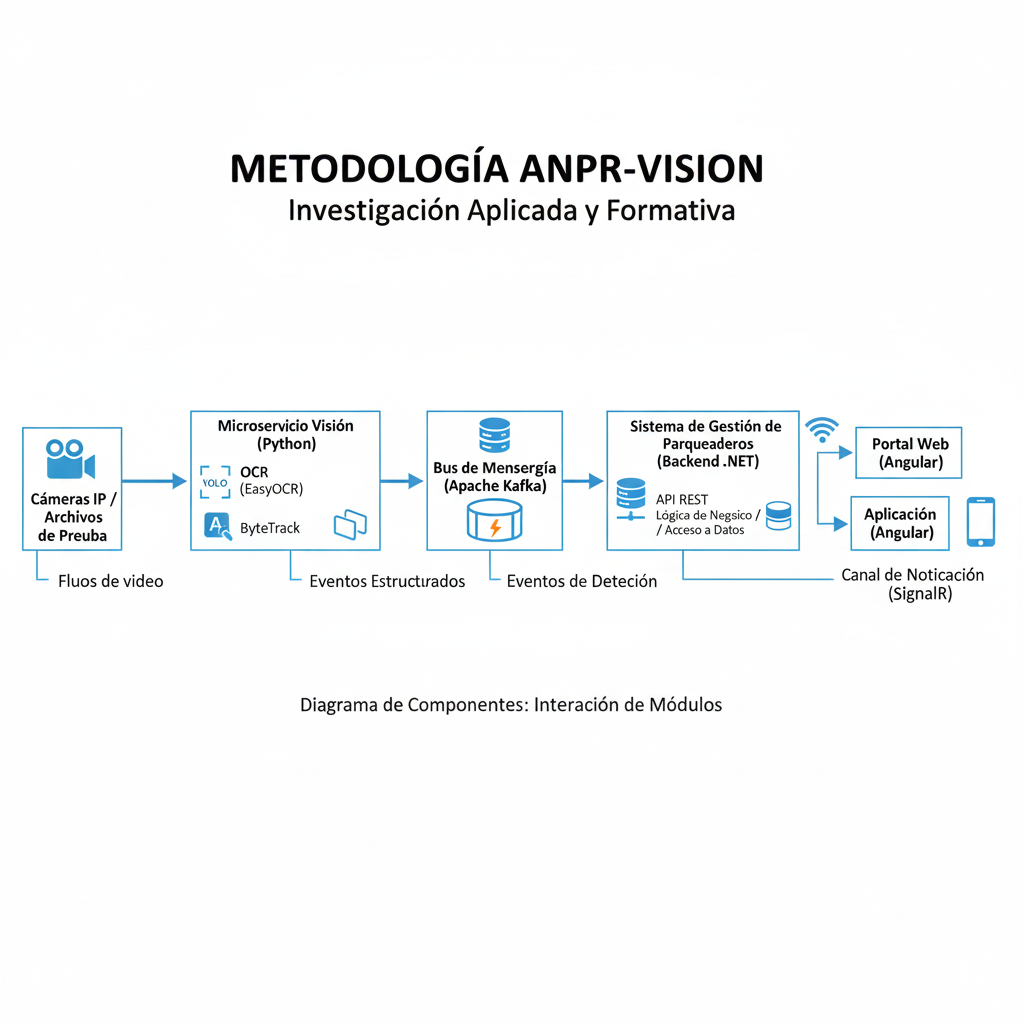
\includegraphics[width=\linewidth]{graphics/metodologia_anpr_vision.png}
    \caption{Arquitectura lógica de ANPR-VISION: flujo de información desde las fuentes de video hasta las interfaces web y móvil.}
    \label{fig:arquitectura_anpr_vision}
\end{figure}
